\section{Data}

% \cite{2015AnA...578A.114F} HIPS

\begin{enumerate}
\item Survey images

  \begin{itemize}

  \item Default: Fermi color image. Mention other survey options

  \item HiPS file format and HEALPix projection for the map

  \item Our images came from CDS' HiPS database of 300+ images

  \end{itemize}


\item Catalog images

  \begin{itemize}

  \item Fermi-LAT - 3FGL and 2FHL

  \item SNRcat

  \item GeTeV Catalogue

  \end{itemize}
\end{enumerate}


\begin{figure}[h]
  \centerline{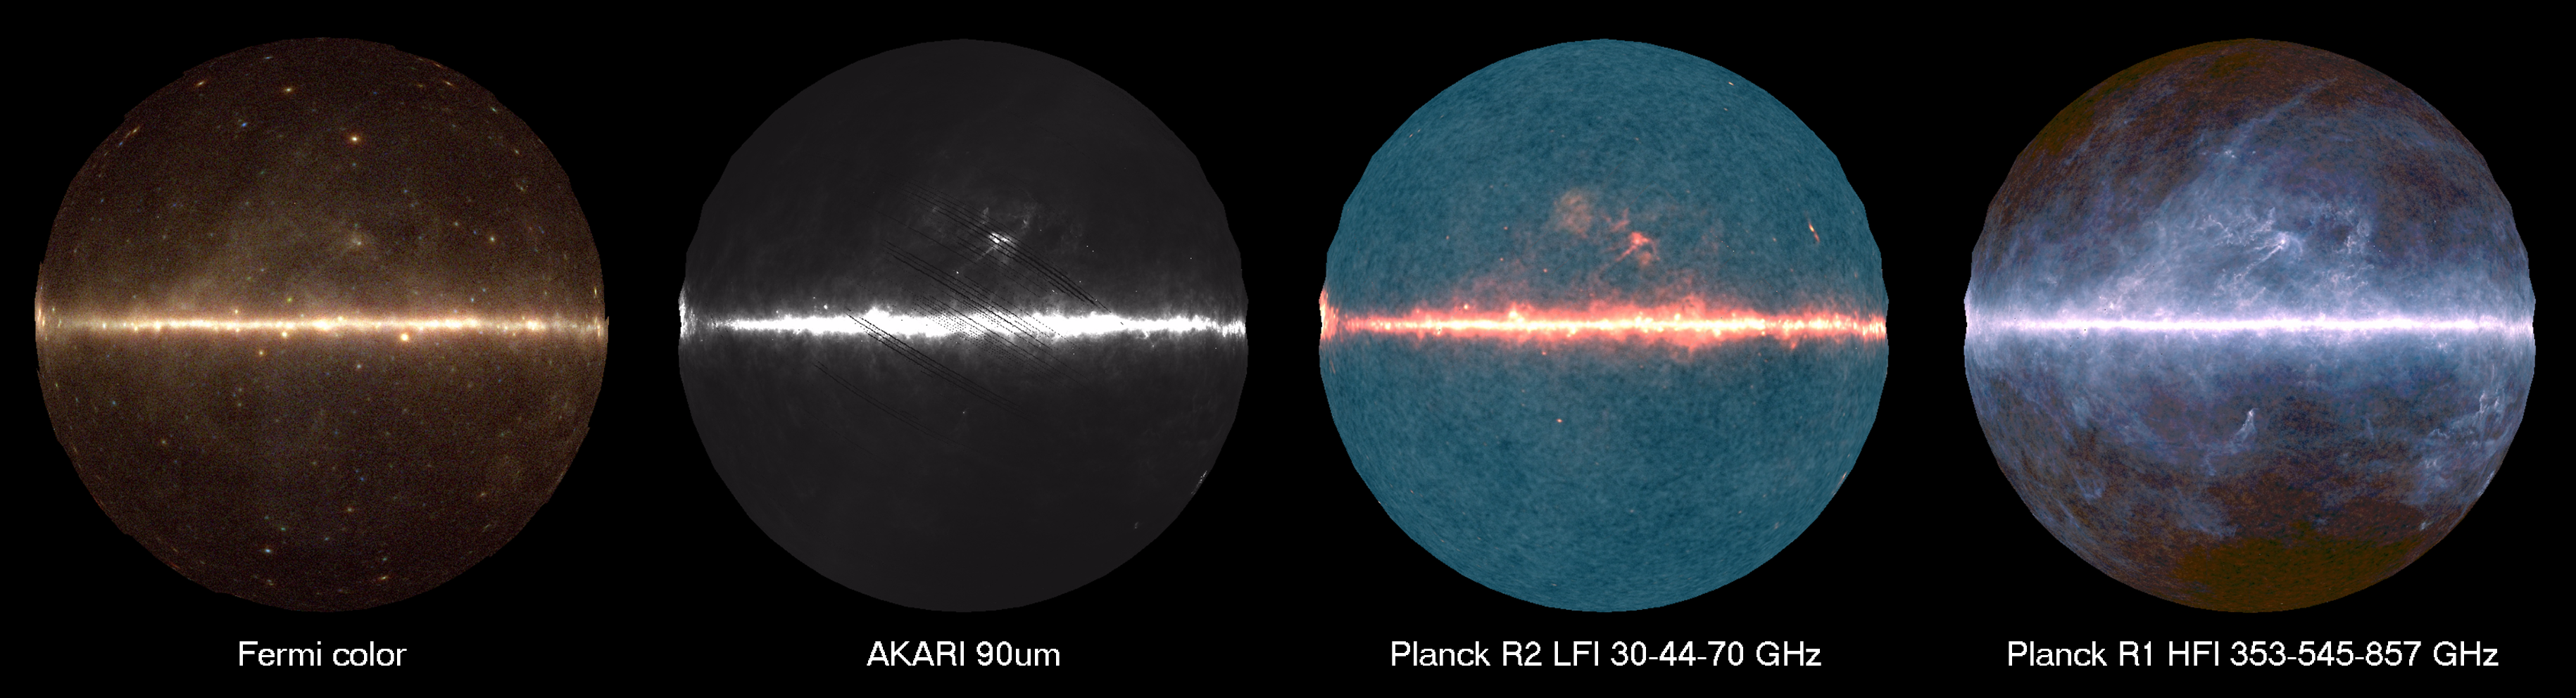
\includegraphics[width=\textwidth]{figures/four_images_captions}}
  \caption{Survey images (left to right): Fermi color, AKARI 90um, Planck LFI, Planck HFI.}
\end{figure}

\begin{figure}[h]
  \centerline{\includegraphics[width=\textwidth]{figures/vela_region_captions}}
  \caption{The Vela Region in various survey images and color maps.}
\end{figure}



% Table
\begin{table}[tb]

\caption{
Source catalogs currently displayed on \gammasky .
We plan to add other catalogs of interest to gamma-ray astronomers in the future,
e.g. the upcoming H.E.S.S. and HAWC TeV source catalogs, or the ATNF pulsar catalog.
}
\label{tab:catalogs}
\tabcolsep7pt\begin{tabular}{ lrll }
\hline
Catalog   & Sources & Updates    & Description \\
\hline
gamma-cat &     153 & continuous & Open TeV gamma-ray source catalog  \\
&&& \gammacat  \\
2FHL      &     360 & fixed      & Second Fermi-LAT catalog of high-energy sources \citep{2fhl}\\
&&& \url{http://fermi.gsfc.nasa.gov/ssc/data/access/lat/2FHL/}  \\
3FGL      &    3034 & fixed      & Third Fermi-LAT point source catalog \citep{3fgl}\\
&&& \url{http://fermi.gsfc.nasa.gov/ssc/data/access/lat/4yr_catalog/}  \\
SNRcat    &     378 & continuous & A census of high-energy observations of Galactic supernova remnants \citep{snrcat}\\
&&& \url{http://www.physics.umanitoba.ca/snr/SNRcat/} \\
\hline
\end{tabular}
\end{table}


%table

\begin{table}[h]

\caption{Image information.}
\label{tab:a}
\tabcolsep7pt\begin{tabular}{ || lrlll ||}
\hline

\textbf{Image} & \textbf{Resolution (arcsec)} & \textbf{Type} & \textbf{Color?} & \textbf{Description}\\ \hline
\textbf{Fermi color} & 51.53 & gamma-ray & color & Fermi-LAT\\
\textbf{AKARI 90um} & 51.53 & infrared & grayscale & AKARI\\
\textbf{CGPS-VGPS CONT} & 51.53 & radio & grayscale & \\
\textbf{Spitzer GLIMPSE360} & 1.2 & infrared & color & Spitzer \\
\textbf{Haslam 408} & 51.53 & radio & grayscale & 408 MHz\\
\textbf{IRIS Band 4-100um} & 51.53 & infrared & grayscale & IRIS \\
\textbf{Planck R2 LFI Color 30-44-70 GHz} & 51.53 & microwave & color & Planck 30-44-70 GHz\\
\textbf{Planck R1 + R2 HFI Color 353-545-857 GHz} & 51.53 & microwave & color & Planck 353-545-857 GHz\\
\hline
\end{tabular}

\end{table}

